\chapter{Implementation}

The previous chapter explained some major design decisions made during this project and this chapter will describe the architecture and implementation details of the resulting application of Secure Dropbox. The implementation language, relevant libraries and implementation platform will be introduced at first. Then the communication pattern of Secure Dropbox KMS and Secure Dropbox client will be explained. The implementation of Secure Dropbox KMS, the Secure Dropbox client and their various components, will be illustrated in detail.

\section{Implementation Dependencies}

\subsection{Secure Dropbox Client}

Both client end and KMS of Secure Dropbox are implemented in Python. To implement the file encryption functions, driver level encryption will be more efficient than user space encryption but might encounter with compatibility problems on different platforms. One reason to choose Python as implementation language is it is an efficient programming language that widely supported to run on most mainstream operating systems like Windows, Linux/Unix and Mac OS X. Moreover it has been ported to the Java and .NET virtual machines already. Program once written could be executed everywhere as long as Python interpreter has been installed. It is a high-level programming language and its libraries and syntax regulation allow developers to implement certain functions with fewer lines of code than in lower level programming language like C. It increases the readability of code and boosts up the programming procedure. Although always being claimed as a scripting language, the object-oriented feature makes Python competent in large scale program implementation as well. Another reason to choose Python is because of its relatively stable version history. Java has 51 different releases for Java SE 6 from 2007 to 2011 and 25 releases for Java SE 7 from 2011 to 2013. However, Python has only 8 versions for Python 2.x in the last 13 years and the latest Python 2.7 has been stable since July 2010. As Secure Dropbox is designed to be a C/S architecture system, a frequently changed implementation platform may cause compatibility problems and make software update routines complicated. Also, Python is the advised programming language by Dropbox to make use of their Core API. Especially, some advanced features are currently only supported by the Python API release like OAuthV2 which performs an indirect Dropbox Authentication during Python API programming. With regard to server end implementation, Python’s powerful web development frameworks like Django or web2py provides mature web development toolkits and libraries to use. Django even automatically provides a well generated back end application console for the web application which reduces development workload tremendously. In conclusion, Python could be an ideal programming language to implement the Secure Dropbox Project.
The implementation platform becomes less important when programming in Python. Python’s interpreter mechanism insures that as long as there is no operating system specified features used in code, the program could be executed everywhere with exact same outcomes. An example of operating system specified feature could be illustrated with the following example which was actually encountered during the Secure Dropbox course project:

\begin{figure}[h]
        \centering
        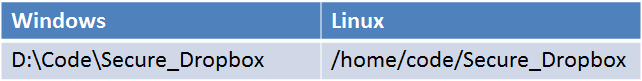
\includegraphics[width=0.7\textwidth]{figures/Representation_of_Path_in_Different_Operation_System.png}
        \caption[Path Representation Schema] {Representation of Path in Different Operating System}
\end{figure}

The two different representations indicate that Windows and Linux are using different symbols as path separator. Assume current working directory is D: in Windows and /home on Linux. For both of them there is a involving some file operations upon a certain file in the folder Secure$\_$Dropbox. When specifying the file path, either ``/'' or ``$\backslash$'' may leads to compatibility issues on different operating systems and file path exceptions. Such problems can be avoided. For example, in Python the path could be generated as follows:

\begin{figure}[h]
        \centering
        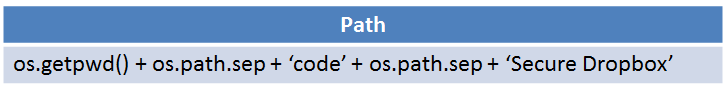
\includegraphics[width=0.8\textwidth]{figures/Platform_Independent_Coding.png}
        \caption[Platform Independent Coding Style] {Platform Independent Coding Style}
\end{figure}

In this way, the variable ``os.path.sep'' will be replaced with ``$\backslash$'' on Windows or ``/'' on Linux by Python interpreter. To make Python program platform independent, any operating system individual features should not appear in the code. It is advised to make more use of the Python OS or other libraries. Secure Dropbox was developed in Windows 7 64-bit operating system but designed as multi operating system usage software. Python 2.7.5 64-bit which was released on May 15th, 2013 was adopted for implementation of both KMS and client. All cryptography modules are generated based on accredited Python cryptography libraries like PyCrypto or M2Crypto.

\subsection{Secure Dropbox KMS}

Secure Dropbox KMS is implemented as a Restful WebService given those desired features. The WebService implementation is based on the Python bottle library which provides ready to use Restful interface for the application.

KMS has been deployed on Ubuntu Server 13.04. Ubuntu Server is currently the most popular guest server platform on the world’s leading public clouds, regarding the total number of instances running or the diversity of customized images available. It offers a complete solution for building highly available, flexible and secure server application production with stable and efficient storage, networking and computation capabilities.

The Ubuntu Server instance with Secure Dropbox KMS Running is currently deployed on the Amazon Elastic Compute Cloud (Amazon EC2). Amazon EC2 is a computing platform which provides resizable compute capacity in the cloud. AS a representational Cloud Infrastructure as a Service (IaaS) cloud platform, Amazon EC2 rents virtual machines with specific computation resources. Also it provides the developers and administrators with the capability of provision processing, storage management, network configurations and other fundamental computing resources to facilitate application deployment and running. Although Ubuntu Server provides monitoring infrastructures, the administration console provided by Amazon EC2 is more intuitive and comprehensive. A sample server monitoring interface is as follows:


\begin{figure}[h]
        \centering
        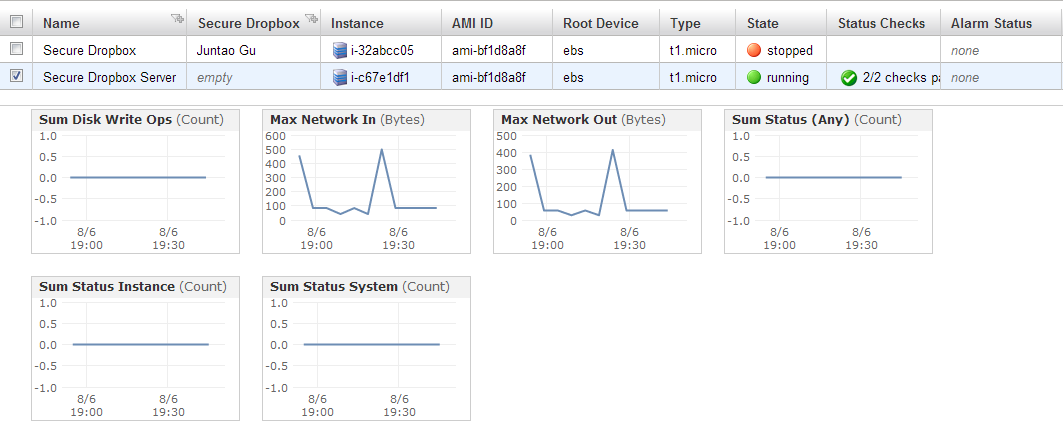
\includegraphics[width=1.0\textwidth]{figures/Amazon_EC2_Server_Monitoring.png}
        \caption[Amazon EC2 Server Monitoring] {Amazon EC2 Server Monitoring}
\end{figure}

Amazon EC2 also offers an intuitive network access control interface. For example, only port 22 is open by default to capacitate the SSH access from any host. Network data flow has been categorized as inbound and outbound direction. Both directions are allowed to be customized by EC2 administrator. For instance, since Secure Dropbox KMS is a restful WebService, all the inbound http requests should be allowed to go through the access control. To customize the schema, the administrator needs to choose the inbound tag, select the rule as custom TCP rule, set any available port number and allow address of 0.0.0.0/0 which means no access control rules on this port. Configuration interface as follows:

\begin{figure}[h]
        \centering
        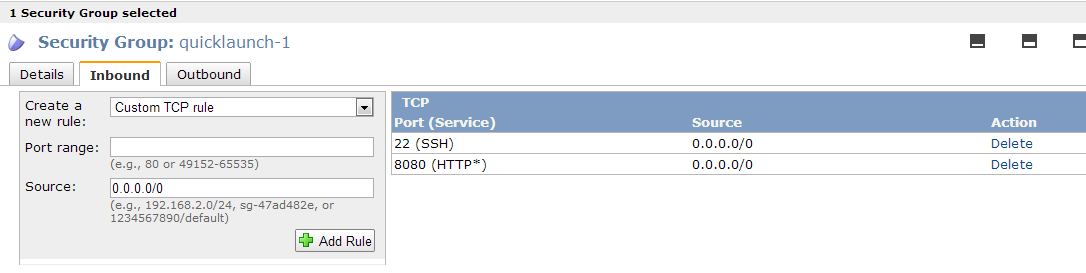
\includegraphics[width=1.0\textwidth]{figures/Amazon_EC2_Security_Group_Customization.png}
        \caption[Amazon EC2 Security Customization] {Amazon EC2 Security Customization}
\end{figure}

To SSH to the Ubuntu Server instance on EC2, An identity based authentication is required. For each cloud application deployed on EC2, a private-key file which associated with the instance will be delivered to the administrator. User is by default granted with root permission if the private-key file is authorized. The following figure indicates the procedure of SSH to Amazon EC2 instance from TCD SCSS Turing service. The SSH command includes a private-key file TRY.pem, a default username ``ubuntu'' and the elastic IP Address of Ubuntu Server Instance. The prompt from the Ubuntu Server instance have no expression about any Amazon EC2 information. Some basic monitoring information like current process number, CPU load and Memory usage will be displayed once login succeeds:

\begin{figure}[h]
        \centering
        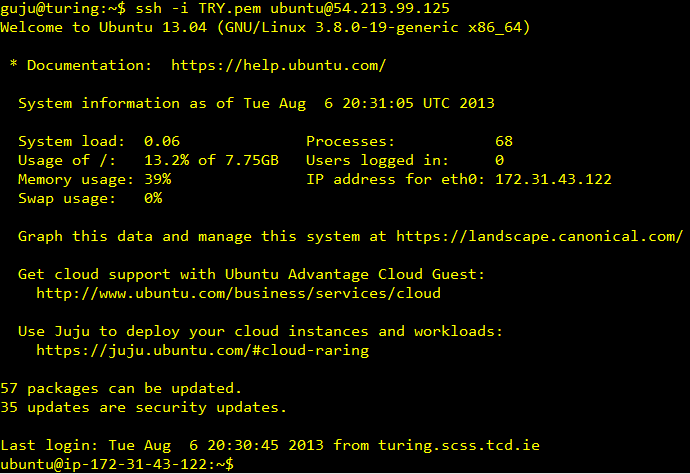
\includegraphics[width=1.0\textwidth]{figures/Amazon_EC2_Instance_SSH_Procedure.png}
        \caption[Amazon EC2 SSH Procedure] {Amazon EC2 SSH Procedure}
\end{figure}

Secure Dropbox KMS uses SQLite as database. SQLite is a SQL database engine delivers file based storage service. It is suitable for building a lightweight disk-based database that does not require a separate server process. The standard python module sqlite3 provides a SQL interface compliant with the DB-API 2.0 specification and a built connection instance that could access to the SQLite database directly.

\section{Communication}

Except the encrypted file instance itself, all information data involves in Secure Dropbox client are downloaded from KMS during initialization and any newly generated data have to be synchronized and permanently stored in KMS. For example, before authentication procedure, the password hash algorithm, salt and iteration time information have to be fetched and the locally hashed password has to be uploaded to KMS again for matching purpose. The communication between the Secure Dropbox client and KMS is performed in REST-style. A typical REST-style architecture generally consists of client end and server end. The client initiates by sending requests to the server. Having received the request, the server will process it and return the corresponding responses to the client. REST requests and responses are generated aimed at the transmission of representations of data resources. Resource to be sent can be essentially any comprehensible and meaningful concept that able to be addressed by both ends. The representation of certain resource is typically a formatted text or document that contains the state or value. In Python programming, JSON is the standard data format that always used for formatting the data to be sent.

To build a REST WebService Server, The python web framework Bottle is used in this project. The Python bottle is a fast, simple and lightweight WSGI micro web-framework for Python. To generate a request routing, a tag with http request method type and desired routine name are proposed as follows:

\begin{figure}[h]
        \centering
        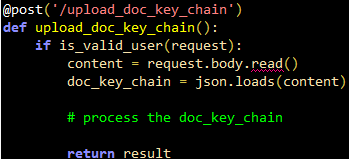
\includegraphics[width=0.6\textwidth]{figures/Restful_WebService_Programming_with_Bottle.png}
        \caption[Restful WebService Programming] {Restful WebService Programming with Python Bottle}
\end{figure}

\begin{itemize}
  \item
  This function will process any POST requests with URL points to the CGI /upload\_doc\_key\_chain.
  \item
  The function ``upload\_doc\_key\_chain()'' is called when such a request arrives.
  \item
  The resource content need to be transmitted and processed is encapsulated in the HTTP body.
  \item
  The resource content has been formatted in JSON so it could be retrieved again if loaded in JSON format.
  \item
  The return value is directly returned to the requester.
\end{itemize}

In the client end, the request is generated as building an http request with required resource data. It could be done with the support of urllib2. It is a standard module in Python 2.7 with definitions of functions and classes which helps in fetching URLs. To call the remote KMS APIs, the target URL should be specified as the routine name that predefined in WebService end. It is simplified by urllib2 to generate an HTTP request and send it to KMS:

\begin{figure}[h]
        \centering
        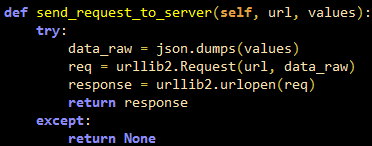
\includegraphics[width=0.6\textwidth]{figures/HTTP_POST_Request_Generation.png}
        \caption[HTTP POST Request Generating] {HTTP POST Request Generating}
\end{figure}

\begin{itemize}
  \item
  The data to be transmitted has to be formatted into JSON
  \item
  An HTTP POST request is generated with data and target URL as parameters
  \item
  The request is sent via ``urllib2.urlopen()'' method and response data received as return value.
\end{itemize}

All communication sessions are initiated by the Secure Dropbox client. Also these data exchanges are designed with no state so that any communication step is atomic and finished in a single session. The request about fetching data will get a response of data instance and request about uploading KMS data will get an error code depends on if the operation succeeds or not.

\section{Secure Dropbox KMS Implementation}

KMS plays a key management processor role in Secure Dropbox. There are three different types of tasks running in KMS: user management, key management and file sharing management. User management processes user’s registration and login requests. Key management mainly performs CRUD operations upon encryption key related issues. File sharing management is responsible for file sharing notification and performing a time task to handle the expired file sharing information. The implementation of some important features and WebService interface will be explained.

\begin{figure}[h]
        \centering
        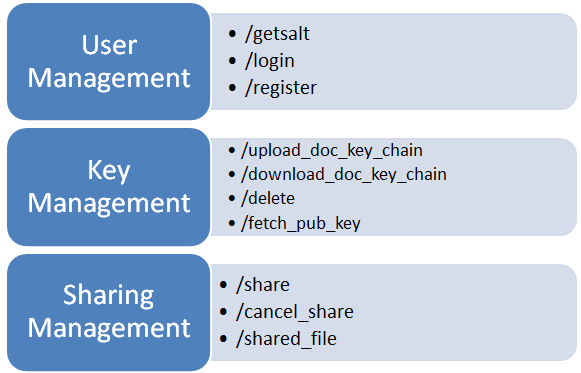
\includegraphics[width=0.7\textwidth]{figures/KMS_Interfaces.png}
        \caption[KMS Interfaces] {KMS Interfaces}
\end{figure}

\subsection{Database Design}

There are three tables in database of Secure Dropbox KMS. The ``user'' table stores user’s username, password and RSA key pairs. User’s RSA public key is recorded in plain text while the private key is stored with encryption. The token is a timestamp to indicate the last login time. The ``key\_chain'' table includes each user’s file encryption keychain which is composed by a unique doc\_id and doc\_key. The doc\_id is guaranteed to be unique since it includes the file owner’s username which is unique defined as public key in the “user” table. Each file has its doc\_id and corresponding doc\_key which is essentially an AES-256 key. The doc\_key is encrypted with the owner’s private key. The ``sharing\_pool'' table consists of sharing information like sharing sponsor and recipient. The doc\_key in sharing\_pool is encrypted with sharing recipient’s public key so that the shared doc\_key could be decrypted with the recipient’s private key. The field URL and expires is generated by Dropbox ``/media'' API. The URL points to the raw encrypted file content and the field expires indicates when the URL turns into not accessible. There is a scheduled task handles the records and deletes those expired records in ``sharing\_pool'' table because certain sharing information becomes useless after getting expired. Logically they should not be able to searched and displayed to the user.

\begin{figure}[h]
        \centering
        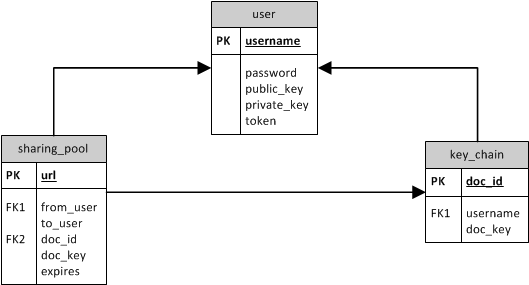
\includegraphics[width=0.8\textwidth]{figures/Database_Design.png}
        \caption[KMS Database Design] {KMS Database Design}
\end{figure}

Although stored in the database of KMS, all these data are generated and uploaded by a Secure Dropbox client. Some essential fields are encrypted with the key not known to KMS but only known to account owner.

\subsection{KMS User Management}

The interface ``@post(/getsalt)'' returns password hash algorithm parameters like algorithm name, salt value and iteration times to Secure Dropbox client. Thus client is able to hash the plain text password with the same parameters as how the hashed password value stored in KMS database was generated. It is called before client performing the login procedure. The function will return a Python dictionary variable like \{``algorithm'': ``sha1'', ``iteration'': 1000, ``salt'': ``vAoH1lpY''\} to the invoker client.

\begin{figure}[h]
        \centering
        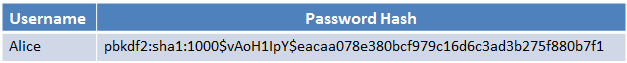
\includegraphics[width=0.9\textwidth]{figures/Hashed_Passwords_in_Database.png}
        \caption[Hashed Passwords] {Hashed Passwords in Database}
\end{figure}

The interface ``@post(/login)'' processes login requests. A login request includes a username and hashed password value. A token of current timestamp will be generated and returned if login information is authenticated or an error code for failed login trials. The user’s RSA key pair is returned as well if login succeeds.

The interface ``@post(/register)'' processes registration requests. All the user information includes username, password and RSA key pair are generated and partially encrypted by the Secure Dropbox client. The KMS server will only check if all the fields meet certain requirements and then perform the storage procedure. Error code returned as registration result.

\subsection{KMS Key Management}

Uploading a new file via Secure Dropbox client is consists of two steps: The first one is encrypting the file and synchronizing it to Dropbox. The second one is uploading the encryption key and other data that involved in the first step to Secure Dropbox KMS. KMS key management module is implemented oriented to the second step.

The interface ``@post(/upload\_doc\_key\_chain)'' receives newly generated doc\_id and corresponding doc\_key. The record will be refreshed if there is one with same doc id exists in ``key\_chain'' table. Otherwise the new doc\_id and doc\_key will be added to the ``key\_chain'' table. Error code returned as uploading result.

The interface ``@post(/download\_doc\_key\_chain)'' returns the keychain which belongs to the user in a Python dictionary format with doc id as key and doc key as the value.

The interface ``@post(/delete)'' receives doc id to be deleted. Not only deleting the record in table key\_chain, it will also trigger the deletion of the corresponding records in the ``sharing\_pool'' table. For example, Alice has a file doc1\_Alice.txt and shared it with Bob. If Alice deletes the record of doc1\_Alice.txt in the ``key\_chain'' table, the sharing information with Bob about this file will be deleted as well. Error code returned as deletion result.

The interface ``@post('/fetch\_pub\_key')'' returns the RSA public key of the user whose name is specified in the request. It happens before users want to share files with the potential sharing recipient. The sharing sponsor has to fetch the recipient’s public key to encrypt the file encryption key before generating that sharing record in ``sharing\_pool'' table. Although the public key is stored in the ``user'' table, it is still designed as part of key management since the RSA key pairs are not involved in user management.

\subsection{KMS File Sharing Management}

The interface ``@post(/share)'' receives file sharing information and stores it into the “sharing\_pool” table. If there is same sharing record in the database then only the doc\_key field will be refreshed to the new file encryption key. Otherwise a new record will be added. An email notification towards the sharing recipient will be created by this method. The example sharing notification is generated as follows:

\begin{figure}[!h]
        \centering
        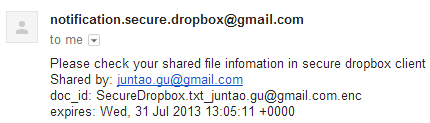
\includegraphics[width=0.7\textwidth]{figures/Sharing_Notification.png}
        \caption[Sharing Notification] {Sharing Notification}
\end{figure}

The notification function could be implemented based on Python smtplib module which defines an SMTP client session object that can be used to send mail.

\begin{figure}[!h]
        \centering
        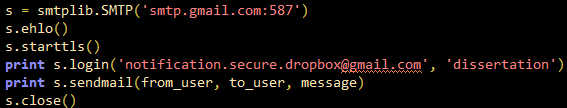
\includegraphics[width=0.9\textwidth]{figures/Sharing_Notification_Implementation.png}
        \caption[Sharing Notification Implementation] {Sharing Notification Implementation}
\end{figure}

\begin{itemize}
  \item
  SMTP (`smtp.gmail.com:587`) generates a SMTP instance encapsulates an SMTP connection to Gmail.
  \item
  ``ehlo()'' identifies the local machine to an ESMTP server.
  \item
  ``starttls()'' puts the SMTP connection in Transport Layer Security (TLS) mode.
  \item
  ``login()'' logins on the Gmail SMTP server with authentication information.
  \item
  Send the mail via ``sendmail()'' method. The message has been generated in the context.
\end{itemize}

The interface ``@post(/shared\_file)'' returns all the sharing records where the to\_user field is the user who is calling this method. A Python dictionary includes doc id, processed encryption key, sharing sponsor, access URL and expiration is returned. This function should be called before the sharing recipient wants to read those shared files.

Since the file sharing URL generated by Dropbox will by default expire three hours later, the sharing recipient would get no access to the URL then. To reduce the confusion, a scheduled task is running as a thread in the server which refreshes the information in sharing\_pool periodically. The task will delete the records in which the timestamp in expires field is later than current timestamp. The refreshing period is by default configured as 600 seconds and configuration interface is open to administrators.

\section{Secure Dropbox Client Implementation}

\begin{figure}[h]
        \centering
        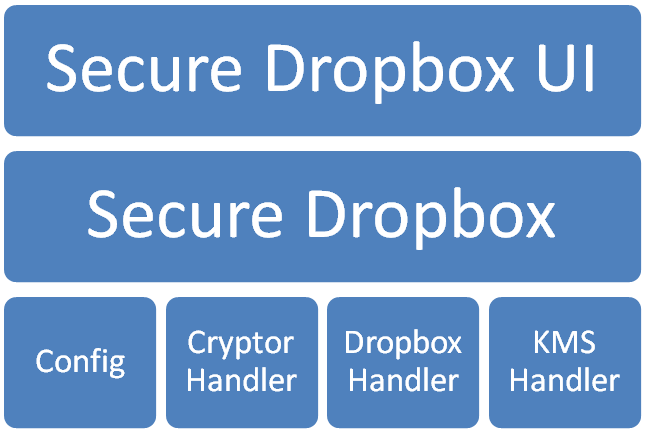
\includegraphics[width=0.5\textwidth]{figures/Secure_Dropbox_Client_Architecture.png}
        \caption[Secure Dropbox Client Architecture] {Secure Dropbox Client Architecture}
\end{figure}

The secure Dropbox client performs cryptography related computations and communicates with both Dropbox and Secure Dropbox KMS simultaneously. In short, according to the architecture diagram above, the Secure Dropbox UI module is responsible for human computer interaction and Application initialization. The secure Dropbox module is the middle ware which controls the data communications and cryptography operations. The judgment of Secure Dropbox module is performed in Secure Dropbox UI module during application initialization. The configuration module includes application environment configuration parameters and it is open to Secure Dropbox User. Cryptor Handler includes AES-256, RSA and other essential cryptography algorithm encryptor instances. Dropbox Handler creates a session handler which is used in Secure Dropbox module when Dropbox file operation or other communication is required. KMS Handler includes the method to communicate with Secure Dropbox KMS. Cryptor Handler is used in KMS Handler as well since some communications between client and KMS requires encryption. Since Secure Dropbox module is an integration of other infrastructure modules, the implementation details will be introduced at last after explaining of those infrastructures.

\subsection{Secure Dropbox UI}

Secure Dropbox is implemented as a command line based application since it performs better platform independency when GUI is not involved. Besides IO function, Secure Dropbox client’s running environment prerequisites are detected and configured during UI initialization. Also Secure Dropbox running mode is decided. The detection procedure is as follows:

\begin{figure}[h]
        \centering
        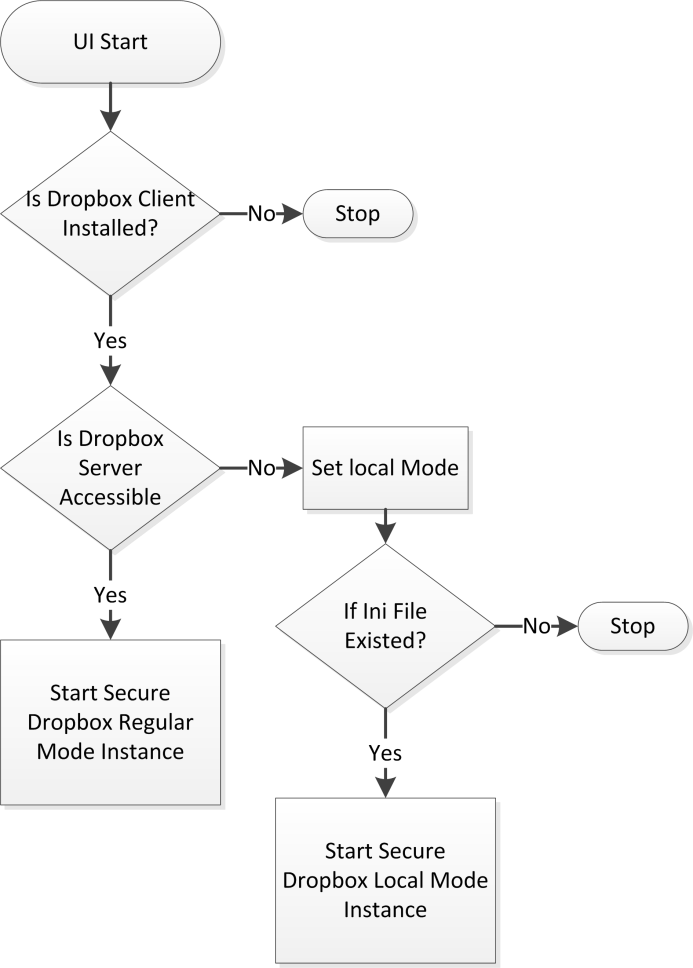
\includegraphics[width=0.6\textwidth]{figures/Secure_Dropbox_Running_Environment_Detection.png}
        \caption[Running Environment Detection] {Secure Dropbox Running Environment Detection}
\end{figure}

If the Dropbox official client is not installed on this computer, the Secure Dropbox client is not allowed to start since no file synchronization operation to Dropbox could be done. The Secure Dropbox will be configured as local mode if either Secure Dropbox KMS or Dropbox server is not reachable. In this situation, if any ini file which works as a local KMS exists, the client will be configured and started in local mode. Otherwise both remote and local KMS will be considered as not available and consequently the Secure Dropbox service is not available. If both Dropbox server and Secure Dropbox KMS are both accessible, client will be initialized in regular mode.

The supported command is different under different mode. For example, under local mode, there are only two commands supported: ``ls'' to print local file list and ``read'' to read local files. However, the supported operations in regular mode are listed as follows:

\begin{figure}[h]
        \centering
        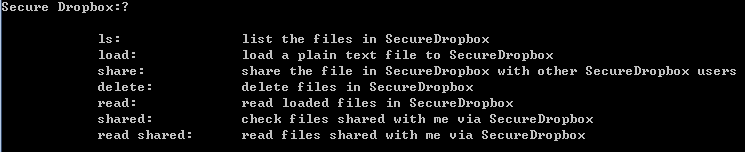
\includegraphics[width=1.0\textwidth]{figures/Supported_Commands_by_Secure_Dropbox.png}
        \caption[Secure Dropbox Commands] {Secure Dropbox Commands}
\end{figure}

The following two examples are print information of command ``ls'' and ``read''. The ``ls'' command lists all local files in the folder named Secure Dropbox in Dropbox application. The sync flag field indicates if the encrypted file’s encryption key could be found in KMS. It might be inappropriate operations that lead to files out-sync. The out-sync file could not be read since no encryption key could be fetched and applied. The second diagram shows the print information of ``read'' command. A ``read'' command automatically invokes the ``ls'' function to display the local file list at first and then show further prompts to guide user to input the sequence number of desired files to be read. It accepts sequence number and reduces the possibility of misoperations by typing file names. The file is stored in cipher locally but decrypted and printed in the same console. It means that the file encrypted by Secure Dropbox could be only read from the Secure Dropbox client. Most user interfaces are designed as the following styles:

\begin{figure}[h]
        \centering
        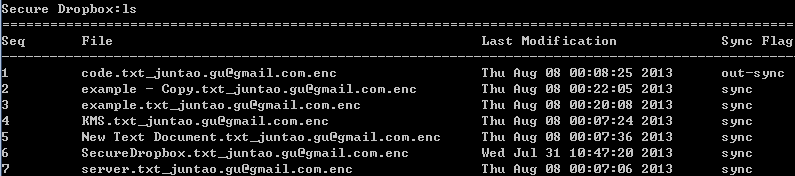
\includegraphics[width=1.0\textwidth]{figures/Command_Print_Information.png}
        \caption[Command Print Information] {``ls'' Command Print Information}
\end{figure}

\begin{figure}[h]
        \centering
        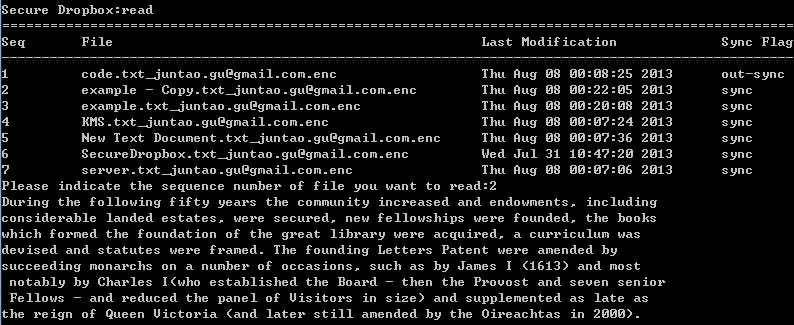
\includegraphics[width=1.0\textwidth]{figures/read_Command_Print_Information.png}
        \caption[Command Print Information II] {``read'' Command Print Information}
\end{figure}

A file loading dialog is provided to choose the file which user wants to upload to Dropbox via Secure Dropbox. It is implemented based on TkInter, a standard Python interface to the Tk GUI toolkit and available on most UNIX platforms, as well as Windows. It facilitates the procedure of specifying the file to be loaded under command line. The return value of the file dialog is a full path of the selected file. Secure Dropbox currently only supports cryptographic operation of text files so any file selected without the suffix “.txt” will be ignored. Also, for access control purpose, the file does not include current user’s account name will be ignored as well. The loading dialog only accepts selection of file instance but not the folder. It is implemented as follows:

\begin{figure}[h]
        \centering
        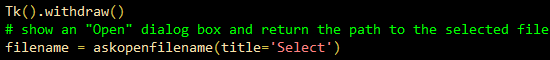
\includegraphics[width=0.8\textwidth]{figures/File_Dialog_Implementation.png}
        \caption[File Dialog Implementation] {File Loading Dialog Implementation}
\end{figure}

\subsection{Dropbox Handler}
Dropbox Core API is used in Secure Dropbox. Only applications that have registered and integrated with Dropbox application console could get an access token to use these APIs. The App key and App secret are generated after registration and they are also key identities when applying for the access token. There are two permissive types of operating Dropbox. Full Dropbox indicates everything inside user’s Dropbox folder is accessible by this application while Application Folder mode indicates the application can only access the specified folder with full permission. Secure Dropbox is using the Full Dropbox permit. Application settings of Secure Dropbox are listed as follows:

\begin{figure}[h]
        \centering
        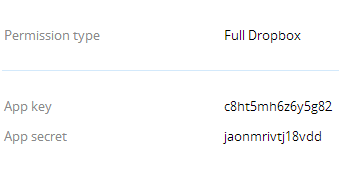
\includegraphics[width=0.6\textwidth]{figures/Application_Settings_of_Secure_Dropbox.png}
        \caption[Application Settings of Secure Dropbox] {Application Settings of Secure Dropbox}
\end{figure}

Dropbox Handler generates an access token via OAuth service of Dropbox. This is an authorization framework that allows a third-party application to obtain access permission for HTTP services that is using this framework. For example, to operate Dropbox, rather than inputting the Dropbox username and password to the third-party application, the user still authenticates on Dropbox and then an access token will be granted to this application if authentication succeeds. Significantly it reduces the security risks for Dropbox since it is difficult to audit if the third-party application code records the user’s username and password. In Secure Dropbox, the Dropbox authentication web page will pop up automatically and wait for user’s authorization action. The permission type is indicated as follows:

\begin{figure}[!h]
        \centering
        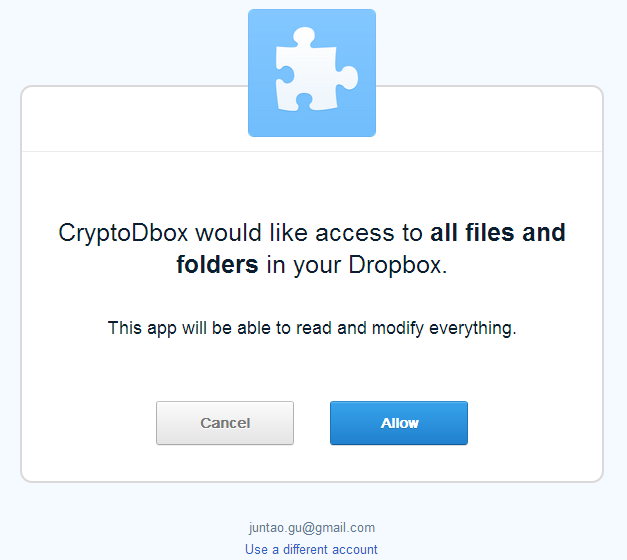
\includegraphics[width=0.7\textwidth]{figures/Dropbox_OAuth_Service.png}
        \caption[Dropbox OAuth Service] {Dropbox OAuth Service}
\end{figure}

Access token will be granted after clicking Allow button. Although Dropbox Core API provides powerful interfaces that sufficient to implement any file operations, Secure Dropbox still relies on Dropbox official application with respect to all file operations for simplification of implementation and robustness of file synchronization mechanism. For now, only file sharing function in the Secure Dropbox client is performed through the Dropbox Core API by calling the ``/media'' interface. It gets a temporary authenticated URL for the target file. A Python dictionary with a URL and expiration information like:

\begin{figure}[!h]
        \centering
        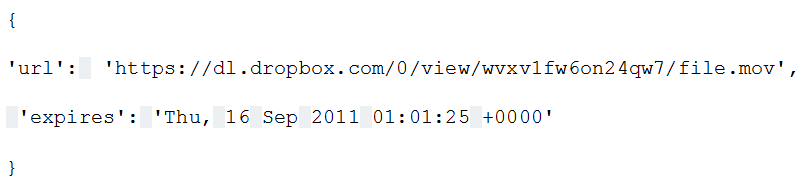
\includegraphics[width=0.9\textwidth]{figures/Return_Value_of_Dropbox_Sharing_API.png}
        \caption[Return Value of Dropbox Core API] {Return Value of Dropbox Core API}
\end{figure}

The expiration time is consistent with the validation of OAuth access token to avoid the situation that the user whose last login has been expired but still able to get access to the file. Secure Dropbox stores this information and notifies sharing recipient. The sharing recipient gets file content by accessing the specified URL and read it after decryption procedures.

\subsection{Cryptor Handler}

Cryptor handler includes implementation of AES-256. It also contains an encapsulated file encryption tool based on AES-256 that is frequently used in the client. The AES-256 is based on interfaces provided by PyCrypto module which also covers some other cryptography algorithms for the Python programming. AES-256 in Secure Dropbox is in CBC mode and configured with both trunk size and initial vector length in 16-bit. RSA encryption/decryption handler is implemented based on M2Crypto. M2Crypto is another popular cryptography library for Python with better padding implementation of RSA algorithm. In Secure Dropbox, pkcs1\_padding mechanism is adopted. AES-256 key generator is implemented in Cryptor Handler while RSA key pair is not generated here since logically it belongs to the registration procedure. Algorithm of generating random AES key is based on plain text file content as random seeds and implemented as follows:

\begin{figure}[h]
        \centering
        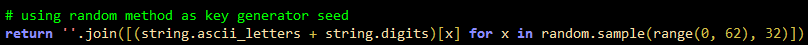
\includegraphics[width=1.0\textwidth]{figures/AES_Key_Generation.png}
        \caption[AES Key Generation] {AES Key Generation}
\end{figure}

\subsection{KMS Handler}
KMS Handler implements communication interfaces with Secure Dropbox KMS. Important features and implementation dependencies has been introduced in the Communication section. It includes a Cryptor instance for some cryptography operation involves in this module. Typically most methods in KMS Handler are related to generating data package to be sent to KMS based on data transferred from Secure Dropbox module. For example, to make a file deletion request to KMS, data package is generated and sent as follows:

\begin{figure}[h]
        \centering
        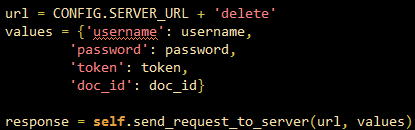
\includegraphics[width=0.6\textwidth]{figures/KMS_Data_Package_Generation.png}
        \caption[KMS Data Package Generation] {KMS Data Package Generation}
\end{figure}

\begin{itemize}
  \item
  The URL is created with a fixed prefix ``CONFIG.SERVER\_URL'' which includes KMS’s IP address and listening port. ``delete'' specify the interface to call.
  \item
  Value to be sent is wrapped as a Python dictionary.
  \item
  ``send\_request\_to\_server'' is called for sending requests. Return value is the response from KMS.
\end{itemize}

KMS interface invoker methods are implemented correspondingly. Some methods are called by Secure Dropbox Module directly while some else are performing as reusable infrastructure methods like ``send\_request\_to\_server()''.

\subsection{Configuration Module}

The configuration module includes Dropbox application settings, running environment settings, cryptography parameters and communication error code. The same error code schema is defined in the KMS side as well so these indicators could be recognized by each other. Dropbox application settings include App key, App secret and access type. Server URL is specified with the combination of IP address, listening port of KMS and the other running environment include like default local location of encrypted files and local KMS file. Cryptography parameters like SHA1 iteration times and encryption block size is defined as well. Secure Dropbox users can change these macros in the configuration file to customize individual security requirement and other settings.

\subsection{Secure Dropbox Module}

SecureDropbox is the main function class in the application. This module includes the user information handler, the Dropbox handler, the KMS handler and the Cryptor handler. The functions provided by these handlers are integrated into Secure Dropbox module to enable Secure Dropbox performing as desired. For example, a file uploaded to Dropbox through Secure Dropbox is encrypted by ``encrypt\_file()'' method of Cryptor handler, uploaded to Dropbox via access token generated by Dropbox handler. Moreover, its encryption key is uploaded to KMS by KMS handler as well. Secure Dropbox is created and manipulated by the Secure Dropbox UI instance. During initialization, it will create a folder in the Dropbox application named Secure Dropbox and all operations done by Secure Dropbox will be only in this folder.

Secure Dropbox has two operation modes. The regular mode works when a normal Internet connection is made. The local mode only supports reading local files. Besides different operations, the user authentication procedure is essentially different. The authentication process in regular mode is performed as described previously while local mode authentication is performed based on the local KMS file. This KMS file is created when login with regular mode and refreshed based on corresponding data in KMS. It actually stores an instance contains user account information, file encryption keychain and RSA key pair information. When the KMS server is not reachable, this information could perform as a read-only local KMS.

\begin{figure}[h]
        \centering
        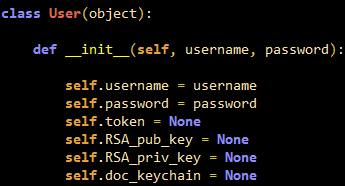
\includegraphics[width=0.5\textwidth]{figures/User_Instance_Stored_in_Ini_File.png}
        \caption[User Instance in Local KMS] {User Instance in Local KMS}
\end{figure}

The local KMS file is created by dumping a User class instance into a file and encrypting it with the user’s password. Inside the class instance, the password is stored in hash value and ``doc\_keychain'' is encrypted with ``RSA\_priv\_key'' which is also ciphered with an AES key derived from password. In Python, to dump an object into a file, the module pickle is widely used. It implements a fundamental solution for serializing and de-serializing objects in Python. To read the local KMS file, a right password as decryption key must be used. Otherwise, the decrypted result of local KMS file will be meaningless that no user instance could be fetched. The input username and password will be matched with that in KMS file. Encrypted file encryption keychain and RSA key pairs will be decrypted and fetched after a successful authentication.

The RSA keys are produced in the Secure Dropbox module with certain interfaces of M2Crypto before uploading registration record. It is made and stored in pem format and then fetched and uploaded with private key encrypted. Coding implementation as follows:

\begin{figure}[h]
        \centering
        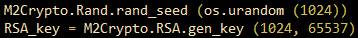
\includegraphics[width=0.6\textwidth]{figures/RSA_Key_Pair_Generation.png}
        \caption[RSA Key Pair Generation] {RSA Key Pair Generation}
\end{figure}

``/media'' is used for generating file sharing record in Secure Dropbox while it causes different characters coding style on diverse of operating systems. In operating system like UNIX or other Unix-like operating systems, the newline character is coded as LF (``0x0a''). However, in Windows it is encoded as LF+CR (``0x0d0a''). The URL generated by ``/media'' points to the file data instance that is located on Unix-like file system on Dropbox which changes the windows coding style into Unix coding style. Since the encryption is done within Windows environment, the binary level change like losing several bytes in the cipher will lead to drastic influences on decryption result. To solve this problem, any ``0x0d0a'' should be replaced with ``0x0a'' in cipher’s binary content as follows:

\begin{figure}[h]
        \centering
        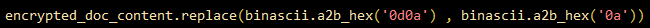
\includegraphics[width=1.0\textwidth]{figures/Replacements_of_Newline_Characters.png}
        \caption[Replacements of Newline Characters] {Replacements of Newline Characters}
\end{figure}
